
\section{Unstructured Data} \label{s:ud}
The awkward term \emph{\ud} is intended to complement the term \emph{\sd}---which commonly refers to data stored in a database (DB) of some variety. Logically, \ud{} can be thought of as all data not stored in a DB, but most commonly it is used to refer to \emph{files} housed in a \hfs{}. Compared to scalars arranged by row and column within a DB, files can be far more expressive, comprising such varied formats as office documents, digital images, and full-motion video, collectively referred to as \emph{rich data types}.

\subsection{Objects} \label{s:obj}
The notion of files is further abstracted to \emph{objects}. While there isn't a canonical definition specifying precisely what constitutes an object in the context of storage, \os{} implementations tend to represent \emph{object} as the union of a data object, \fsm{} and (user created) \cmd{}.

Here \emph{data object} is simply the user data; for example a Microsoft Word document that contains a travel itinerary. The \emph{\fsm{}} may include things such as the name of the file, the time it was created and when it was last updated. Thus far a basic \fs{} would suffice to house both the data (the Word document) and \fsm{} (the filename, time created, etc.). An \os{} provides the ability to add a third element, \emph{\cmd{}}, to the mix.

\Cmd{} allows the user to annotate the base data with arbitrary text, often in the form of key-value pairs. Continuing our example, when storing our travel itinerary in an \os{} we may want to annotate this document with select key data such as: Year=2013, Department=Sales, Territory=US, Status=Approved.

From this example we see that \cmd{} provides a mechanism to make the core file more useful by allowing the user to abbreviate the file with select information that can later be used to logically group documents. Additionally we can perform a lightweight search against the \os{} for all travel requests by Sales in 2013 that were approved for travel within the US and quickly return a list of all objects that meet these criteria.

This is exactly the type of function we'd expect to perform against a sophisticated RDBMS. However, instead of being restricted to storing scalars, we gain the full expressiveness possible with rich data file types without sacrificing the ability to convert that data into information through mechanisms such as the ability to perform predicate searches. Better still, searching \md{} stored within the \os{} is a far lighter weight operation than searching the full content of every file stored and attempting to piece together logical groupings ad hoc. The value \md{} brings to \ud{} is substantial. In short, it's \md{} that allows us to add structure where none would otherwise exist in the \ud{} world. In \S\ref{s:md} we describe this value more deeply.

\subsection{Data Growth}
Throughout the last two decades a recurring topic in IT is how to manage the exponential increase in the volume of data that must be stored as societies move increasingly to a digital world \cite{Gartner:2010:IT}. What's more, while the growth of data to date has been tremendous, the rate of increase is projected to grow greater still. IDC projects that the \emph{ Digital Universe} will grow by a factor of 300---to 40,000 exabytes!---by 2020, and that enterprises will have ``liability or responsibility for 80\% of the information'' in this digital universe. Further, \ud{} is expected to constitute 90\% of the 40,000 exabytes \cite{IDC:2012:DigitalUniverse}.

This staggering growth correlates to a shift from text to rich data types such as digital images and video. To get a sense of \emph{how} such data growth can be rationalized, in \cite{RJP:2012:SDVSUD} we see where the capacity required to store a high definition movie trailer is 20,000 times greater than that required to store a traditional movie review. It's this continued shift to rich data types that fuels such spectacular growth; and this growth shows few signs of subsiding.

\subsection{Data Containers}\label{s:dc}
Such growth begs the question: where are we to store this mountain of data? While RDBMS are used to hold \sd{}, \fss{} and \oss{} are common containers for unstructured data.

Much of the R\&D over the last 50 years for \fss{} has focused on how to improve storage efficiency (e.g. optimizing \fs{} overhead), durability, and reliability. However, from the perspective of user interface, the basic paradigm of the \hfs{} remains largely unchanged since its introduction in the 1960s.

For enterprise-class \oss{}, a cardinal focus has been on answering the question: How do we achieve extreme scale beyond that provided by traditional \fss{}? Since their genesis, the target market for \oss{} has been massive data stores, where the feature of cataloging all objects stored has greater value.

It's comparatively easy to keep track of thousands of files for a few years; it's far more difficult to manage billions of them for decades. The Internet and the falling price of magnetic storage have shifted our expectations of digital storage. We now expect data to live in perpetuity, instead of being periodically culled for usefulness. This new behavior further highlights the need for large-scale data management both from a capacity and file count standpoint.

A common misperception is that \oss{} are a replacement for \fss{}; instead, they are an augmentation. The \fs{} is tightly coupled to the operating system and provides a well established mechanism for organizing files within a hierarchy of directories. By contrast, an \os{} focuses on changing the presentation layer to the storage consumer through a simplified interface while achieving enormous scale by aggregating many \fss{} into a single, higher-order grouping.

Figure \ref{fig:stack} presents an abstract view of the storage stack on a single node. The function of each superior layer is to aggregate and abstract the layer beneath, permitting greater sophistication and specialization in each layer without increasing complexity to clients of upper layers. The object storage layer creates a \emph{distributed storage service} to client \apps{} without requiring the clients to manage data distribution.

\begin{figure}[h]
  \centering
    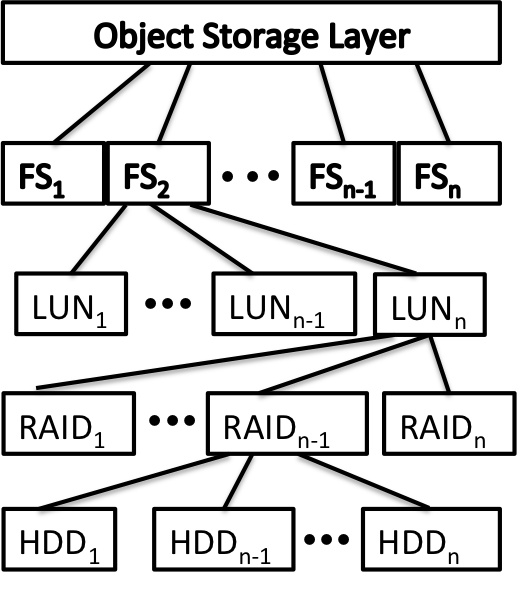
\includegraphics[width=0.3\textwidth]{fig/os-view.png}
  \caption{Storage Stack}
  \label{fig:stack}
\end{figure}
